\documentclass[tikz,border=2pt]{standalone}
\usepackage{amsmath}
\usepackage{amssymb}
\usepackage{pgfplots}
\pgfplotsset{compat=1.18}
\usetikzlibrary{arrows.meta}
\begin{document}
% Table 5.3: of the nine outcome combinations of (P) and (D) exactly four occur: optimal/optimal, P unbounded/D infeasible,
% P infeasible/D unbounded, both infeasible. Strong duality removes four cells, weak duality removes unbounded/unbounded.
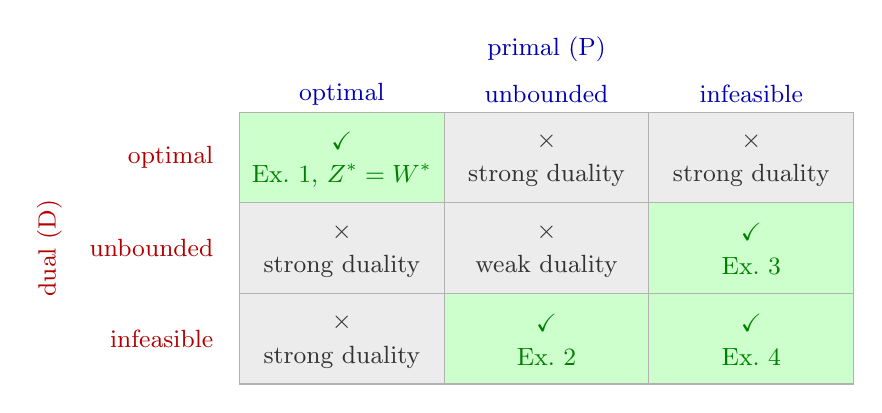
\begin{tikzpicture}[font=\small, >={Latex[length=2mm]}, x=2.6cm, y=1.15cm]
  % column (P) and row (D) headers
  \node[blue!70!black, anchor=south] at (1.5,0.45) {primal (P)};
  \foreach \lab [count=\c] in {optimal, unbounded, infeasible}
    \node[blue!70!black] at (\c-0.5,0.2) {\lab};
  \node[red!70!black, rotate=90, anchor=south] at (-0.82,-1.5) {dual (D)};
  \foreach \lab [count=\r] in {optimal, unbounded, infeasible}
    \node[red!70!black, anchor=east] at (-0.08,-\r+0.5) {\lab};
  % possible cells: (column, row, example)
  \foreach \c/\r/\ex in {1/1/{Ex.~1, $Z^{\ast}=W^{\ast}$}, 3/2/{Ex.~3}, 2/3/{Ex.~2}, 3/3/{Ex.~4}} {
    \fill[green!20] (\c-1,-\r+1) rectangle (\c,-\r);
    \node[green!50!black] at (\c-0.5,-\r+0.68) {$\checkmark$};
    \node[green!50!black] at (\c-0.5,-\r+0.3) {\ex};
  }
  % impossible cells: (column, row, reason)
  \foreach \c/\r/\why in {2/1/strong, 3/1/strong, 1/2/strong, 1/3/strong, 2/2/weak} {
    \fill[gray!15] (\c-1,-\r+1) rectangle (\c,-\r);
    \node[gray!40!black] at (\c-0.5,-\r+0.68) {$\times$};
    \node[gray!40!black] at (\c-0.5,-\r+0.3) {\why\ duality};
  }
  % grid
  \draw[gray!60] (0,0) grid[xstep=1, ystep=1] (3,-3);
\end{tikzpicture}
\end{document}
